\label{sec:sliceID}
\subsection{Event Slicing and Cosmic Removal in Pandora}

The work presented in this note relies on the Pandora approach for event reconstruction~\cite{bib:pandoraub}. The scope of Pandora is to do the low-level pattern-recognition step of the reconstruction, i.e. group hits into clusters, clusters into particles and particles into hierarchies. 

\subsubsection{Slicing \textcolor{green}{Wouter}}
After the hit creation, the Pandora Cosmic Pattern Recognition is run over all hits, aiming to construct muon tracks and associated delta showers. At this stage, obvious cosmic activity is tagged using geometric information. Now, the obvious cosmic tagged hits are discarded and the filtered hit collection enters a next stage, slicing. A "slice" is a subset of hits which are topological distinct. It is assumed that different slices correspond to different particle hierarchies. Each slice is now reconstructed both under the cosmic hypothesis and the neutrino hypothesis. A typical event contains approximately 5 slices.

\subsubsection{Clustering and Vertex Finding \textcolor{green}{Wouter}} 
Pandora starts by running the 2D clustering on the hits in each slice and in each plane separately. Then, a number of 3D candidate vertices is created by finding positions that project down on to the ends of the 2D clusters we have made so far. All of these candidates are fed into the support vector machine (SVM) vertex selection, and the most appropriate one is chosen. This 3D vertex is used to split any existing clusters that straddle the vertex. Then, the cluster matching algorithms are run, where the clusters are compared between views and modified to improve the matching.

\subsection{SliceID : Cosmic Removal through topology and scintillation-light \textcolor{green}{Wouter}}
\label{sec:sliceID:SliceID}
\par After the Pandora pattern-recognition algorithm suite has isolated individual interactions into reconstructed \emph{slices} and removed those that are either through-going or out-of-time, the remaining task is to identify which (if any) slice is associated to a neutrino interaction. This is done by relying on scintillation light information to reject slices incompatible with light recorded in-time with the beam. Additionally, topological cuts aimed at rejecting stopping-muon events which enter the TPC are used. The SliceID is at the core of all neutrino selections performed in this analysis, and serves as the first, common step in the analysis, responsible for the majority of cosmic-rejection.
\\
\par We have three handles that we use to distinguish between neutrino and cosmic-ray slices.
\begin{enumerate}
    \item Simple optical pre-selection cuts - is the slice totally inconsistent with the beam flash?
    \item Topological score - to what extent does the slice look like a neutrino interaction in the TPC?
    \item Flash-matching score - to what extent does our flash-hypothesis for this slice match the beam flash?
\end{enumerate}
To select the neutrino slice, or reject the event at this stage, the following procedure is followed:
\begin{itemize}
    \item Insist that there is a beam-triggered flash in the beam window.
    \item Only consider slices that pass the optical pre-selection cuts.
    \item If the slice with the largest topological score in the event remains, then select it as the neutrino.
    \item If not, then choose the remaining slice with the largest flash-matching score.
\end{itemize}
\begin{figure}
    \centering
    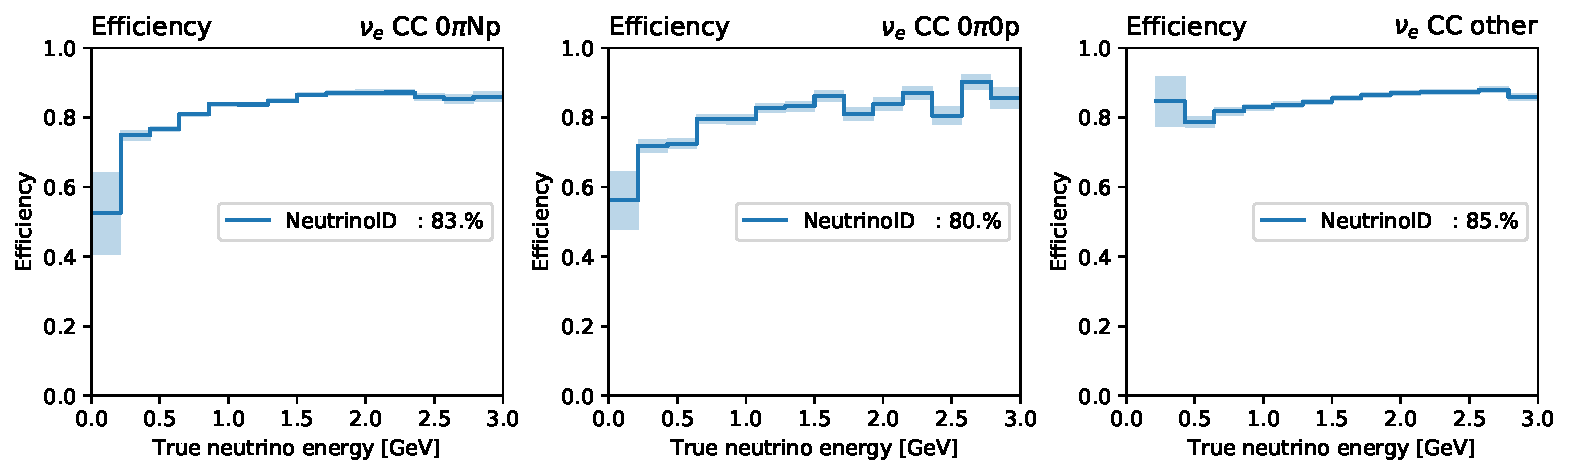
\includegraphics[width=\textwidth]{NuId-Ch2/Images/efficiency_cat_0.pdf}
    \caption{The performance of the SliceID in function of the true neutrino energy for the channel with protons (left), the channel without vertex activity (middle) and events with pions in the final state (right).}
    \label{fig:sliceid}
\end{figure}

The performance of the SliceID for electron neutrino simulated events is given in~\cref{fig:sliceid}.

\subsection{CRT Veto and Distance Tagger \textcolor{green}{Elena}}
\label{sec:sliceID:CRT}
Contrary to  $\nu_\mu$ interactions and cosmic rays, the charged particles associated to $\nu_e$ interactions are unlikely to deposit energy in the Cosmic Ray Tagger (CRT). Building upon this discriminating factor, the CRT Veto and CRT Distance Tagger are preselection tools which leverage the additional CRT information available for Run 3+ data.
When used, these CRT tools are applied at the pre-selection stage in the following order: CRT Veto, SliceID, CRT Distance Tagger. The CRT tools are especially impactful for the 1e0p channel, where discrimination handles based on the proton PID are obviously missing. \\


\emph{CRT Veto.} %On average, only one in six events passing the MicroBooNE common optical filter is associated to beam-induced activity. The remaining events are triggered by activity that originates outside the TPC: either external beam induced activity or cosmic rays. %Given the $\mathcal{O}(10)$ cosmic ray muons in each drift window, this equates to a starting signal-to-background of $\sim 1 : 60$.
%The CRT Veto reduces these backgrounds by looking at CRT activity in time with the beam window. 
%The CRT Veto looks at CRT activity in time with the beam window. 
The CRT veto looks for a time coincidence between the scintillation light recorded in time with the 1.6 $\mu$s beam-spill (beam-flash) and a CRT hit: if a CRT hit occurs within a 1 $\mu s$ of the beam flash, the event is rejected. For this coincidence, only CRT hits with PE $>$ 100 pe are considered; we do not apply a constraint on the position of the flash nor on the position of the CRT hit. 
The rejection power and efficiency of the CRT veto are calculated using the BNB external and the $\nu_e$ overlay samples, respectively. The BNB external passing rate is $\sim$59\%,  and the $\nu_e$ efficiency greater than $\sim$94\% for all electron neutrino energies, raising at low energies. \\


\emph{CRT Distance Tagger.} 
The CRT Distance Tagger tool builds upon the standard pandora neutrino vertex reconstruction and the CRT tagging of TPC tracks. A TPC track is tagged with a CRT hit association if the track projection onto a CRT panel and a CRT hit are close in space. 
To perform this association, the track projection to the CRT is calculated under the hypothesis that the associated particle crossed the TPC at the time registered by the CRT hit under consideration; more details on the CRT hit to TPC track match are available in \cite{bib:CRTPresel_Technote}.  The CRT Distance Tagger checks the minimum distance between the reconstructed neutrino vertex and each track tagged with a CRT hit. If the minimum distance is less than 14 cm, the event is rejected. An example event tagged by this cut is shown in Figure~\ref{fig:crtdist00}.  For the CRT Distance Tagger, the BNB external passing rate is $\sim$81\%,  and the $\nu_e$ efficiency greater than $\sim$96\% for all electron neutrino energies, raising at low energies. \\
 
\begin{figure}[h!]
\centering
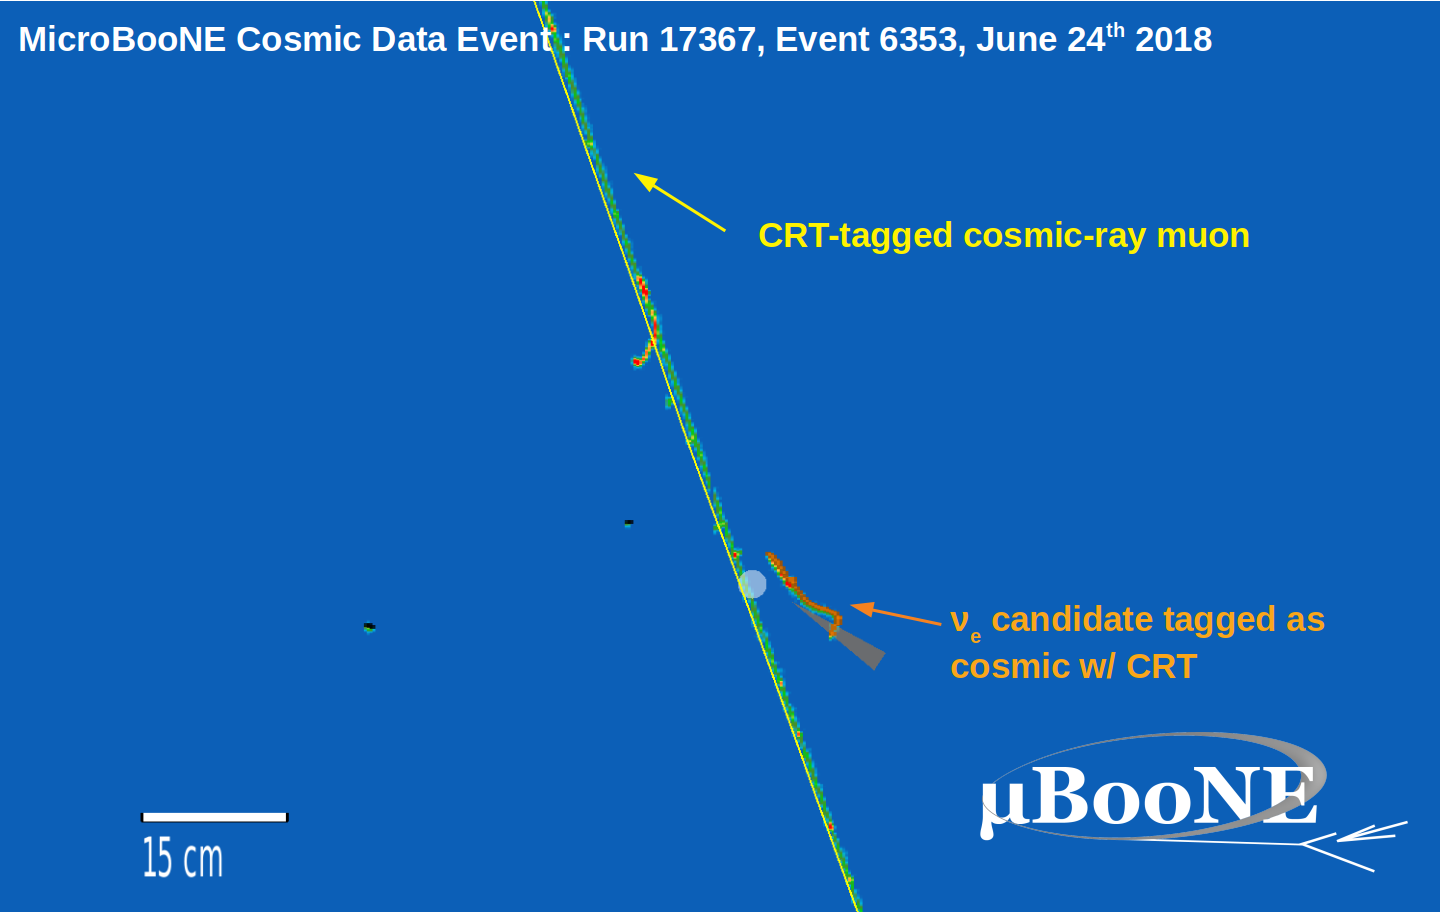
\includegraphics[width=0.4\textwidth]{NuId-Ch2/Images/crttagger_01.png}
\caption{Example $\nu_e$ candidate tagged as cosmic thanks to the CRT distance tagger. From the event one can see that the reconstructed EM shower is associated to EM activity associated to the incoming muon.}
\label{fig:crtdist00}
\end{figure}

An overview of the impact of the CRT on cosmic rejection can be seen in Figure~\ref{fig:crt} where the beam-time distribution for the $8E18$ POT Run 3 open dataset is shown after SliceID (left), and after SliceID and CRT cosmic-tagging tools (both CRT veto and distance tagger) have been applied (right), with EXT backgrounds dropping by more than a factor of 3.
Further details and a preliminary study of the CRT  impact on an electron neutrino preselection can be found in \cite{bib:CRTPresel_Technote}. 

\begin{figure}[ht] 
\begin{center}
    \begin{subfigure}[b]{0.45\textwidth}
    \centering
    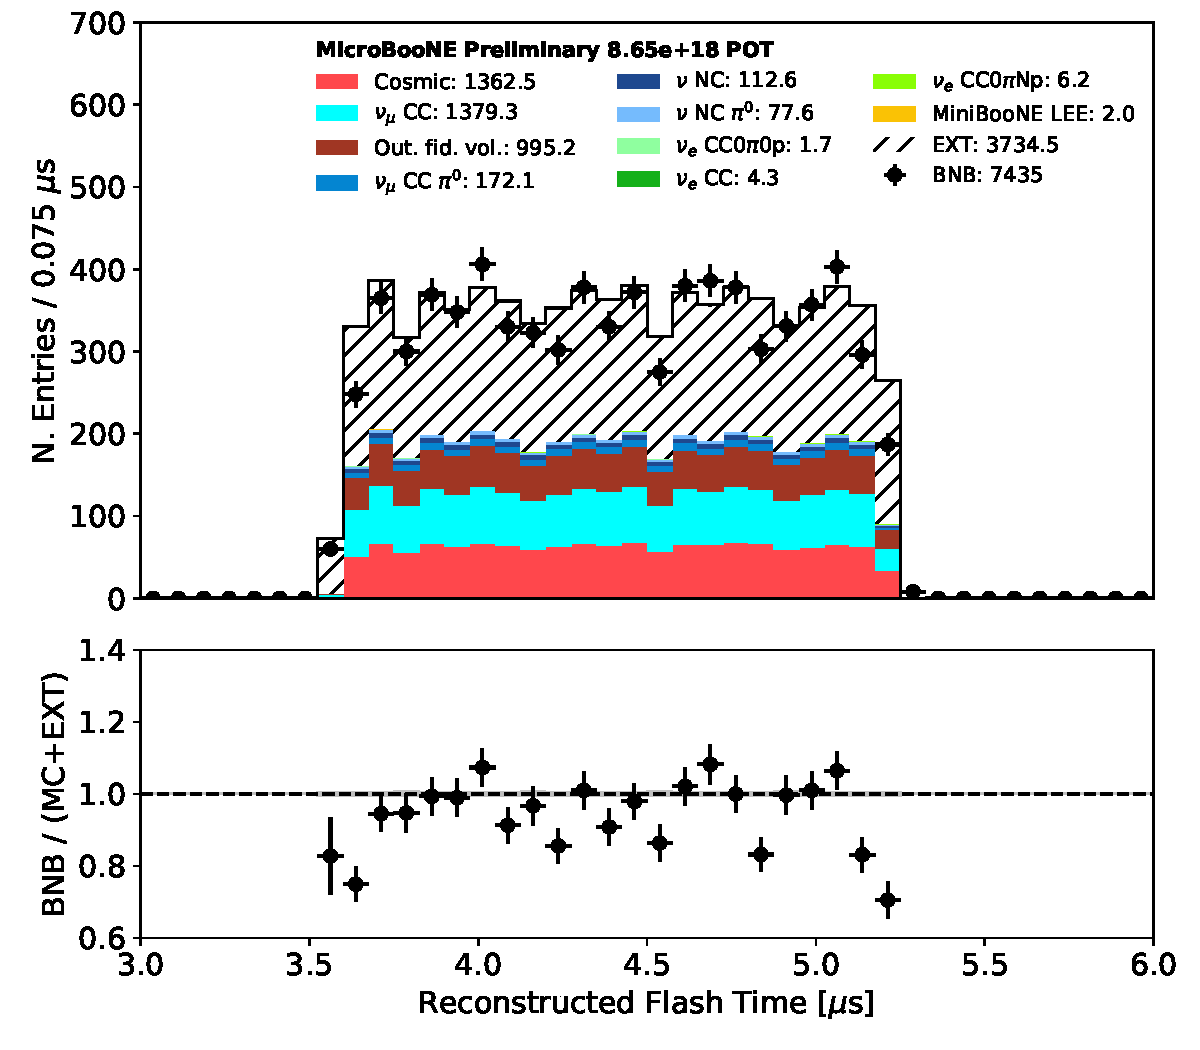
\includegraphics[width=1.00\textwidth]{NuId-Ch2/Images/flash_time_01152020.pdf}
    \caption{\label{fig:crt:pre} no CRT tools.}
    \end{subfigure}
    \begin{subfigure}[b]{0.45\textwidth}
    \centering
    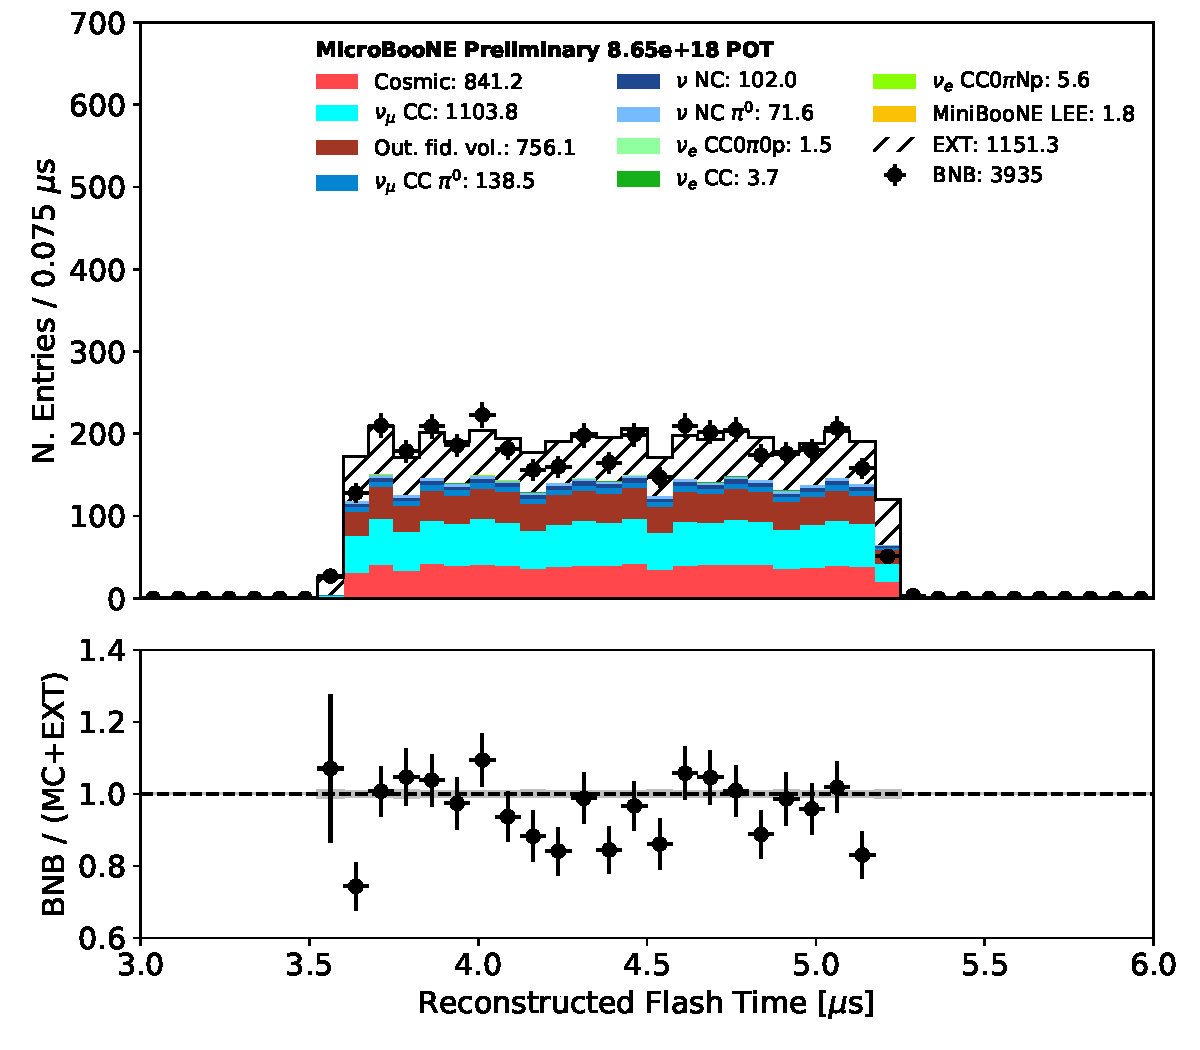
\includegraphics[width=1.00\textwidth]{NuId-Ch2/Images/flash_time_01152020_CRT.pdf}
    \caption{\label{fig:crt:post} with CRT tools.}
    \end{subfigure}
\caption{\label{fig:crt} Beam timing distribution before (left) and after (right) CRT tools have been applied. The EXT contribution is reduced by over a factor of three.}
\end{center}
\end{figure}